\documentclass[letterpaper,10pt,serif, draftclsnofoot,onecolumn, compsoc, titlepage]{IEEEtran}

\usepackage{graphicx}
\usepackage{listings}
\usepackage{amssymb}
\usepackage{amsmath}
\usepackage{amsthm}

\usepackage{alltt}
\usepackage{float}
\usepackage{color}
\usepackage{url}

\usepackage{balance}
\usepackage[TABBOTCAP, tight]{subfigure}
\usepackage{enumitem}
\usepackage{pstricks, pst-node}

\usepackage{geometry}
\geometry{margin=.75in}

\usepackage{hyperref}
\usepackage{verbatim}
\usepackage{listings}

\title{The STEM Academy Data Solution}
\author{Progress Report \\ Shannon Ernst, Kyle Nichols, Javier Franco\\ 7 December 2016\\ CS 461 Fall 2016\\ Group 48}

\begin{document}
\maketitle
\begin{abstract}
It has been a term of foundation building for the STEM Academy Data Solution. The project was assigned, requirements were outlines and a design has been produced. Though much work is left to do, this document outlines the current progress.
\end{abstract}
\newpage
\section{Purpose and Goals}
The STEM Academy program in Corvallis, Oregon, seeks to provide education in science, technology, engineering and math to the K-12 community through various programs, campus, and clubs.
They are self funded, relying on grants, donations and other sources, many of which require results-based data on the success of STEM Academy programs.
This data is collected from surveys that participants take while they are enrolled in one of STEM Academy's camps and other programs.
Currently, these surveys are administered on paper and the responses are tabulated by hand by volunteers.
This has not been an effective way of collecting current data to help secure funding and many of the surveys go untabulated.
The STEM Academy does have the ability to register participants online through Ideal Logic, but this is this does not help them with tabulating survey data.
They need a system which will allow them to electronically create surveys, a database to house all of the data from those surveys, and a report generation system so they can view the most current data in a timely and meaningful way.

A website which will allow the STEM Academy to create and distribute surveys, as well as view helpful data results, is the best solution.
The website should allow them to create questions that can be included across multiple surveys.
The questions should be able to be templated so that only one part of the question need change according to the topic of the survey.
Surveys should be able to be distributed via a web link or printed.
After a survey is taken, the data should be stored in a database according to the type of program.
This data should be queriable based on custom queries.
The user should be able to make a query based on the question and collected demographics as well as filter by program.
This service should be user friendly; the user should not need to know any SQL or other querying language in order to get data from the database.
After a query, the data should be able to be saved and added to a printable report so that it can actually be used in grant proposals and marketing material.
This website will be an all in one package for collecting and reporting on data in a timely fashion which is what the STEM Academy truly needs.
By the Engineering Expo, we will be able to present this website and show the full path of data collection, from creating the survey to querying to report generation.

\section{Weekly Progress Summary}
\subsection{Shannon Ernst}
\subsubsection{Week 1}
This week I contacted Central Services as we had not heard from them.
Our ticket had been lost.
They told us that we can work on a LAMP stack and extend the preexisting domain for the STEM Academy.
This means that the code would be done in PHP and MySQL.
There is nothing inherently wrong with this as we were intending on using these any way for our database management.
We also established a weekly meeting with our client for Tuesday at 9 am.
The next steps are creating the website through Central Services.
\subsubsection{Week 2}
This week we met with our client to show a basic mock of what we are doing for the web app. The demo was basic HTML with no 
functionality aside from some links to different pages to simulate functionality. 
We are going to continue working primarily in HTML for the moment.
Central Services says we can do the LAMP stack which is what we are going to go with however they have not gotten back to us.
Goals for the coming week is to have a better html frame work so we can illustrate the flow of the program to the client.
We will then work on functionality.
\subsubsection{Week 3}
This week I started implementing functionality for adding questions to the survey.
\begin{figure}
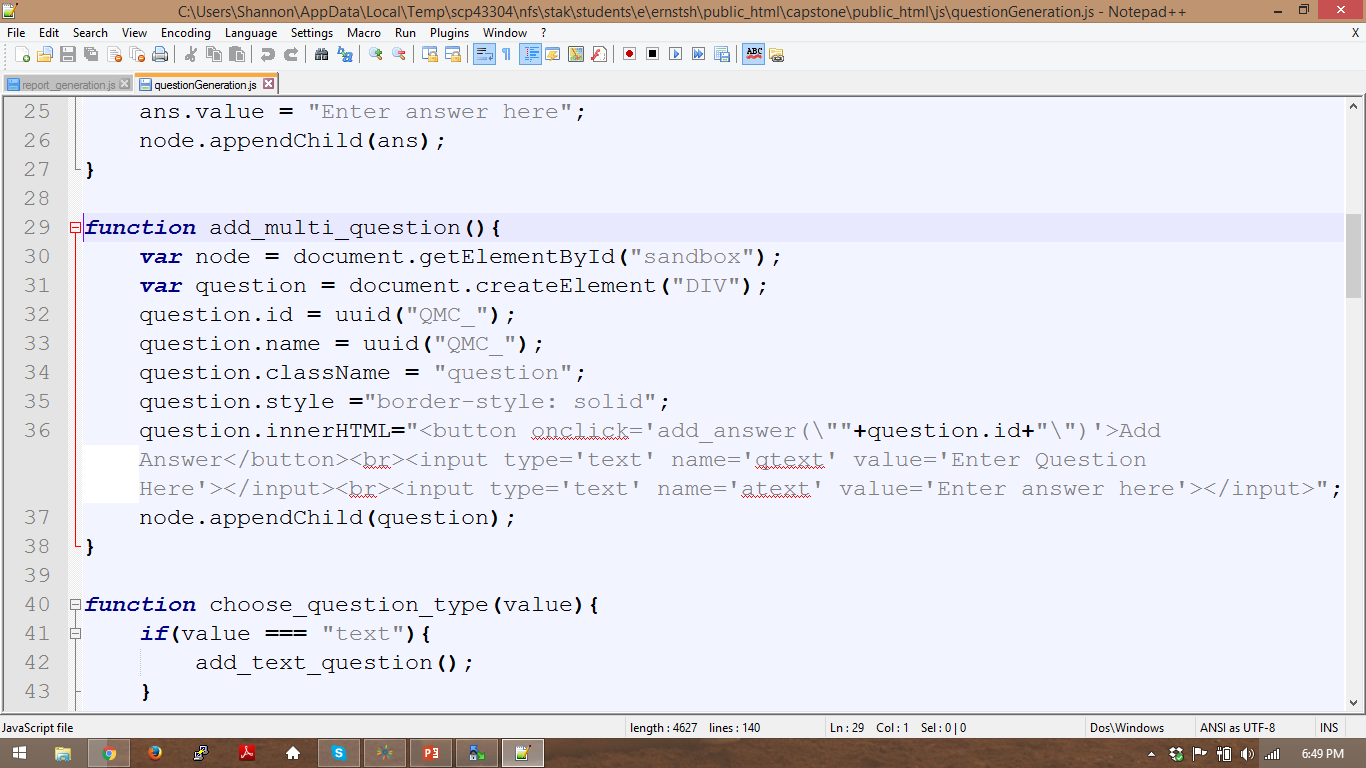
\includegraphics[scale=.5, width=\textwidth]{code_snippet_1.png}
\caption{This code is an example of the DOM manipulation process of adding a question to the survey generator.}
\label{fig:code1}
\end{figure}
Figure 1 is an example of the code I worked on. I am using DOM manipulation to add questions to the survey creator as we
don't know how many questions the admin is going to want to add and they should be able to add as many as they want. These 
should come up at the click of a button. In this case of adding a multiple choice question, I add it to the sandbox and give it some
ids so it can be identified on the page. I then add the inner html which will initially provide a place for getting the question text 
and a place for getting one answer. There is also a button to add answers to this particular div. We pass in the id of the div to 
know what question that answer corresponds to. 
Over the weekend I'm going to continue working on this as well as implementing preview survey.
I need to call Ideal Logic to figure out how to export enrollments so that we can associate them with camps to set up our new log in
functionality. Instead of distributing surveys via links we are going to do it via the students selecting their camp and then themselves from the enrollment list. 
\subsubsection{Week 4}
This week I implemented the beginnings of survey creation.
\begin{figure}
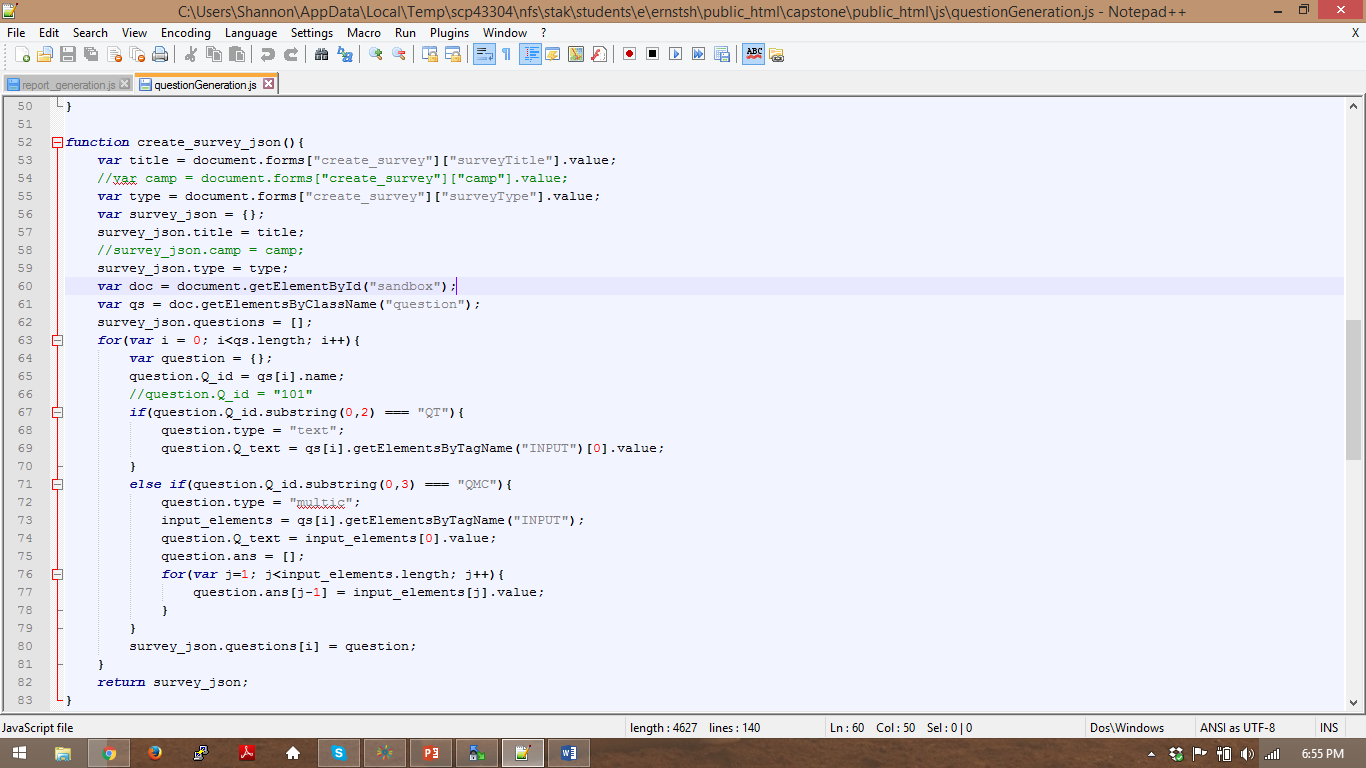
\includegraphics[scale=.5, width=\textwidth]{code_snippet_2.png}
\caption{This code is an example of the DOM manipulation process of adding a question to the survey generator.}
\label{fig:code2}
\end{figure}
Figure 2 illustrates how I have constructed the json and to generate questions dynamically and create surveys.
I still need to be able to recall surveys, save and edit preexisting ones.
I still need to call Ideal Logic. We met with our client this week to demo and provide updates.
All is going well.
\subsubsection{Week 5}
This week we contacted central services to get the sub domain.
We are working on getting php working for posting json.
We sketched a query structure with the client.
This coming week we will do the progress report and wrap up alpha with successful PHP POSTs.

\subsection{Javier Franco}
\subsubsection{Week 1}
This week I looked at creating an alternative design for creating the search form since I thought that my previous design would not work.
The new design is based on selecting a question to query first for a survey.
Then selecting an operator for the query and specifying a value that is going to be queried through a drop down menu or by manually entering a value.
I compared this design idea to Qualtrics and noticed that it uses this set up.
I also studied the operators that Qualtrics uses for the different types of questions that a user will be able to create and how it carries out multiple field queries.
The plan for next week is to start developing our webpages, so that we can have something to show to the client and I will also be studying more on how to use Angular JS 2 to get a better understanding.
\subsubsection{Week 2}
My plan for next week is to create a weekly schedule and to set aside 4-6 hours a day to work on the project to better manage my time and to make progress on the project.
This week I watched another tutorial video on Angular 2 and I worked on creating query form page, but encountered errors while trying to query the clubs, camps, and programs for the drop down list.
I created three tables for the club, program, and camp that I need to include in Kyle's database.
I felt that I was not as productive as I should have been and I will make it up by working on the project over the weekend.
\subsubsection{Week 3}
This week I added some functionality to the report form generation page.
The page now allows a user to delete/add a query.
I also created the functionality that allows administrative users to login/logout.
Some issues that I faced this week was that by not having the appropriate properties on the files and folders it effected the results produced by the .js and .php files which took me a while to figure out.
My plan for the weekend is to add more functionality to the page by allowing a user to select a camp and a survey to query.
\subsubsection{Week 4}
This week I was able to get the adding a camp page to work and an issue that I encountered was that it was time consuming finding the error that caused it because webpages are hard to debug.
Our group met up with the clients and I now have a better understanding of the things they want to be able to query.
However, I am worried that it will be difficult to come up with a good design that satisfied their demands for the report generation webpage.
For the upcoming week I will be focusing more on the part of the project that I am responsible for and my goals for the week is to complete the query functionality for a survey.
\subsubsection{Week 5}
This week our group met up with the client and they gave me feedback on my report generation design.
I am going to have to change my design in order to meet their requests of the stuff they want to be able to query.
The plans for the upcoming week are to create the demo video, make revisions on our documents, make a progress report, and also work on the capstone project.
For the upcoming week I am worried that I will not have time to work on the capstone project since we have to make revisions to our documents, make a progress report, and a demo video.
I will also be having a midterm for Linear Algebra that I need to study for.

\subsection{Kyle Nichols}
\subsubsection{Week 1}
The first thing I did for the project was over winter break by setting up a prototype database on ONID.
I did this through creating the tables as outlined in the design document: Survey, Question, Contains, Responder, Student, Parent, Response, Multiple\_Choice, Text, and Matrix.
These tables were created empty.
I did not yet add any example data to the database.
The ultimate plan was to store the database somewhere provided by Central Services, but since we still had not heard back from them, I still needed something so as not to lose forward momentum.
\subsubsection{Week 2}
The next week, I created the initial setup of our web page and handed it off to the others to create their pages, starting with some basic templates and functionality.
This template-like code came from what I had created for another class at my Engineering public\_html/ space (located at web.engr.oregonstate.edu/~nichokyl).
This allowed us to have a place to create some prototype code and my team mates followed with their own public\_html/ pages.
We still stored all of our web service code in public\_html/ in our github directory, but used our own Engineering web pages to test our code for each of our purposes.
At this point, most links went to blank pages, though the page for adding questions and surveys did allow for filling in survey text, but could not save anything or create more than one question.
\subsubsection{Week 3}
During this week I updated the database to include a Camp table based on discussing the needs of the database with the client.
In particular, they needed a way to organize surveys as based on camp.
My original design of the database only accounted for Surveys in a general sense and not their use in camps more specifically.
This also required that I create an S\_Use table to account for the many-to-many relationship that Surveys are used in Camps and Camps use surveys.
Some other modifications were also made to tables based on this change, such as adding and removing attributes.
Plus, I added more demographic information to some tables based on an example survey the client provided: gender and parental income.
\subsubsection{Week 4}
This week I wrote the basic code for adding to the database and selecting from a database.
To do this, I used the mysqli object in PHP and connected it to my personal ONID database.
\begin{lstlisting}
   \$conn = new mysqli("oniddb.cws.oregonstate.edu", "nichokyl-db", "password", "nichokyl-db");
   \$result = \$conn->query("INSERT INTO `nichokyl-db`.`Survey` (`survey\_id`, `title`) VALUES (NULL, '".\$survey->\$title."')");
\end{lstlisting}
I started this component using hard-coded table entries (i.e. the survey->title variable in the example above was given a value of "Example" before insertion) while Shannon was setting up the JSON creation that I would parse from.
\subsubsection{Week 5}
On Sunday of week five, I worked with my group to make progress on creating interaction between survey generation and adding those surveys to a database.
This included creating the code that would parse from the JSON objects provided by survey generation to insert to the database.
The SQL query code seemed to work on adding to tables in the database, but we ran into a problem where POST data PHP wanted to use was empty, so nothing could actually be parsed from it.

\section{Retrospective}
\begin{center}
    \begin{tabular}{ | p{5cm} | p{5cm} | p{5cm} |}
    \hline
     Positive & Delta & Action \\ \hline
	We have a weekly meeting with our client so we are able to iterate quickly & We need to do a better job of following up with Central Services and other outside entities & To fix the follow up problem we will set aside a weekly call time to place these phone calls to get the answers we need \\ \hline
  	We are doing well at keeping up with the coding, much of the functionality is in place & We are not good at meeting with our TA (people sometimes miss the meeting) and we often miss the Friday deadline for the blog posts, updating them on Saturday instead & To change this, we will set better alarms and reminders to make sure we are keeping up with these adminstrative tasks \\ \hline
    \end{tabular}
\end{center}

\section{Current Status}

\subsection{Shannon Ernst}
The survey generation can currently allow the user to add a title, select if it is a pre or post survey, add text questions and add multiple choice questions. The survey can be previewed in a seperate window as well. This means that we are currently successful in dynamically manipulating the DOM of the page and generating the appropriate json to view a survey. The save feature is being debugged. There is a place to associate the survey with the camp. We also have the login established thanks to Javier and the overall flow of the web app is complete.  
\subsection{Javier Franco}
The report generation page currently allows a user to select a camp and returns all of the camp's surveys. There are three sets of radio buttons for specifying the type of query, result, and survey. Based on the type of query that is selected the "Add Query" button adds a query template based on the selection along with a functioning delete button for removing the query. The "Reset" button for the page removes all of the query templates currently on the page and the "Exit" button redirects the user back to the dashboard.

\subsection{Kyle Nichols}
Currently, the database is within the organization it will need to be at.
There may still be some changes to the database once we have fully coded the interaction with the database, as some organization needs for possible queries may not exist.
However, this changes should be minor and consist mostly of superfluous or missing attributes or a need for other relations that don't exist.
Some sample data exists in the database, but this is arbitrary data.
I have some example surveys from STEM Academy, but this have not been added to the database while kinks are still being worked out.

Unfortunately, we currently have not resolved the issue wtih POSTing the JSON objects to the PHP file that adds to the database.
This is preventing us from implementing full interaction between the database and other components, at least in a secure way.
However, in the mean time, I have a temporary fix for this issue:
If a .json object exists in the same directory as the source code inserting into the database, I can get the contents of that file and store that in a JSON object to be parsed.
This is not how we will want to implement the JSON transfer in the final version, but for now I can use this to get insertion into the database functional while we continue to test our POST issue.
I can create example .json files to implement the parsing of JSON objects for insertion or selection data for the SQL queries.
In addition, Shannon and Javier can create .json instead of using POST until we resolve the issue with POST.

\section{Left to Do}

\subsection{Shannon Ernst}

The survey generation is functionally mostly done. The primary issues at the moment are saving and some functional UI components
such as moving questions, deleting questions and developing the matrix question. The functional UI components will not be difficult to implement as the matrix question is pretty much the same code as the multiple choice with some changes and moving questions requires more DOM manipulation. Deleting a question is going to be a little tricky as via DOM manipulation you need to delete from 
the parent node which may not always be clear. Saving the surevy has been the top priority as we have not been able to get the 
json to be decoded correctly on the PHP side to insert things into the database. This is a major blocker as we will be posting many 
json objects to alter the database. The next steps once saving is complete is to clean up the UI from a css perspective and make sure the surveys are being recalled 
correctly from the database. Once we know how to successfully pass around json between client and server, the hard work is done.
\subsection{Javier Franco}
The things that remain to implement for the report generation page include returning a query result when the Submit button is clicked and displaying the result of the query in an empty form that will allow a user to add a caption to the result.  In addition, I need to implement saving the report results into the database and also allowing a user to return to those results to make additional queries or changes. I also need to add check boxes for the demographic information incase the user wants to breakdown the query result information. Once I get the query results working for one camp I will have to make adjustments to make the report generation page work for multiple camps. 

\subsection{Kyle Nichols}
The database organization is good and there are no current plans to change it considerably.
Some changes may continue to occur as we continue to develop our service and test it.
Several issues have occurred already where modifications needed to be made, and more may still happen.
Howver, looking forward and the work left to do on database interaction, the connection between the survey generation and report generation components and the database needs to be implemented fully.
Currently, the code for generating SQL queries is written, but it is basic and does not take requests from other pages for queries.
The code will needed to be expanded, taking in JSON objects and parsing those objects to know what kind of query or queries are being requested (i.e. a \emph{SELECT} or \emph{INSERT} and what information to send in those queries.

\end{document}
